\documentclass[usenames, dvipsnames, spanish, aspectratio=169]{beamer}

\usetheme[progressbar=frametitle]{metropolis}
\usepackage{appendixnumberbeamer}
%\usepackage{draftwatermark}
\setbeamercolor{background canvas}{bg=}%transparent canvas

%\setbeamertemplate{itemize items}[ball]
%\setbeamertemplate{itemize subitem}
\beamerdefaultoverlayspecification{<+->}
%\usepackage[utf8]{inputenc}
\usepackage[T1]{fontenc}
\usepackage{fontspec}
\usepackage{float}
\usepackage{tcolorbox}
\usepackage{lipsum}
%\usepackage{fourier}

\usepackage{xcolor}
\usepackage{booktabs}
\usepackage[scale=2]{ccicons}
\usepackage{hyperref}
\usepackage{pgfplots}
\usepgfplotslibrary{dateplot}

\usepackage{animate}
\usepackage{xspace}
\newcommand{\themename}{\textbf{\textsc{metropolis}}\xspace}

\usepackage{tikz}
%\usepackage{media9}
\usepackage{multimedia}
\usepackage{multicol}
\usepackage{animate}
\usefonttheme{professionalfonts}

\newcommand{\quo}[2]{{\raisebox{.2em}{$#1$}\left/\raisebox{-.2em}{$#2$}\right.}}
\newcommand{\llav}[1]{  \left\{#1\right\} }
\newcommand{\pic}[1]{  \left\langle #1\right\rangle }
\newcommand{\conv}[1]{\xrightarrow[ \hspace{0.15cm} #1  \hspace{0.12cm}]{}}
\newcommand{\norm}[1]{  \left\|#1\right\| }
\newcommand{\pare}[1]{\left(#1\right)}
\newcommand{\corch}[1]{  \left[#1\right] }
%\newcommand{\abs}[1]{  \left|#1\right| }
\newcommand{\ul}[1]{  \underline{#1}}
\newcommand{\dis}[1]{\displaystyle{#1}}
\def\cle{\preccurlyeq}



\usepackage{charter}
\usepackage[utopia]{mathdesign}


%\documentclass[xcolor=dvipsnames]{beamer}
\usepackage[utf8]{inputenc}
\usepackage{color}
\usepackage{braket}				% Notacion braket
\usepackage{amsfonts}
%\usepackage{amsmath}
%\usepackage{amsthm}
\usepackage{graphicx}
\usepackage{subfigure}
%\usepackage{enumitem}   			% para que me aparezca el (i) cuando enumero
\usepackage[shortlabels]{enumitem}
\usepackage{caption}
%\usepackage{subcaption}
\usepackage{float}  				% me deja poner el grafico [H]
\usepackage{mathtools} 			% align
\usepackage{import}
\usepackage{lmodern}				% que hace esto?
\usepackage{cleveref}
\usepackage{bbm}					% lo necesite para usar la funcion indicadora
\usepackage[margin=20pt,font={small,it},labelfont=bf]{caption} % captions 
\usepackage{epigraph}				% para poner quotes 


% \DeclareMathOperator{\constW}{c_1}  % Constante teo principal
% \DeclareMathOperator{\constC}{c_2} % Constant of the power n
% \DeclareMathOperator{\constR}{c_2} % lower bound, == Constant of the power n
% \DeclareMathOperator{\constG}{c_2}    % arc-lenght, == Constant of the power n 
% \DeclareMathOperator{\constF}{c_3} 	% arc-lenght
% \DeclareMathOperator{\constS}{c_4}  % k-nn
% \DeclareMathOperator{\constT}{c_5}  % k-nn
% \DeclareMathOperator{\constZ}{c_6}  % Constante teo principal
% \DeclareMathOperator{\constA}{c_7} % Chuck
% \DeclareMathOperator{\constB}{c_8} % Chick
% \DeclareMathOperator{\constN}{c_9} % lema spacing
% \DeclareMathOperator{\constM}{c_{10}} % lema spacing
% \DeclareMathOperator{\constL}{c_{11}} % Lema restriccion a un entorno
% \DeclareMathOperator{\constP}{c_{12}} % Upper bound
% \DeclareMathOperator{\constQ}{c_{13}} % lower bound 
% \DeclareMathOperator{\constX}{c_{14}}  % lema spacing manifold
% \DeclareMathOperator{\constH}{c_{15}} % arc-lenght proof
% \DeclareMathOperator{\constI}{c_{16}} % arc-lenght proof
% \DeclareMathOperator{\constJ}{c_{17}} % arc-lenght proof
% \DeclareMathOperator{\constY}{c_{18}}  % Constante teo principal






%\usepackage[dvipdfmx]{media9} % only for latex->dvipdfmx


\numberwithin{equation}{section}

\newcommand{\red}[1]{{\color{red} #1}}
\newcommand{\blue}[1]{{\color{blue} #1}}
\newcommand{\green}[1]{{\color{green} #1}}
\newcommand{\cyan}[1]{{\color{cyan} #1}}
\newcommand{\hdiv}{\vskip\baselineskip\hrule\vskip\baselineskip}
\newcommand{\doublehdiv}{\vskip\baselineskip\hrule\vskip1mm\hrule\vskip\baselineskip}

\definecolor{purple}{rgb}{0.9,0,0.8}
\newcommand{\purple}[1]{{\color{purple} #1}}
\definecolor{gray}{rgb}{0.7,0.7,0.7}
\newcommand{\gray}[1]{{\color{gray} #1}}

\newcommand{\hl}[1]{\emph{\purple{#1}}}
\newcommand{\td}[1]{{\red{\bf [#1]}}}
%\newcommand{\note}[1]{{\blue{\textup{[#1]}}}}


\newcommand{\abbr}[1]{{\sc\lowercase{#1}}}



\newtheorem{thm}{Theorem}[section]
\newtheorem{cor}[thm]{Corollary}
\newtheorem{lem}[thm]{Lemma}
\newtheorem{ppn}[thm]{Proposition}
\newtheorem{xc}[thm]{Exercise}
\newtheorem{conj}[thm]{Conjecture}
\theoremstyle{definition}
\newtheorem{defn}[thm]{Definition}
\newtheorem{ex}[thm]{Example}
\newtheorem{remark}[thm]{Remark}
\newtheorem{assumption}[thm]{Asumption}
\newtheorem{claim}[thm]{Claim}
%\newtheorem{problem}[thm]{Problem}
\newtheorem{question}[thm]{Question}

\newcommand{\beq}{\begin{equation}}
\newcommand{\eeq}{\end{equation}}

% ----- ALPHABETS -----

% Greek
\newcommand{\al}{\alpha} \newcommand{\Al}{\Alpha}
\newcommand{\be}{\beta} \newcommand{\Be}{\Beta}
\newcommand{\gam}{\gamma} \newcommand{\Gam}{\gamma}
\newcommand{\ep}{\epsilon} \newcommand{\Ep}{\Epsilon}
\newcommand{\vep}{\varepsilon}
\newcommand{\de}{\delta} \newcommand{\De}{\Delta}
\newcommand{\iot}{\iota} \newcommand{\Io}{\Iota}
\newcommand{\lm}{\lambda} \newcommand{\Lm}{\Lambda}
\newcommand{\ka}{\kappa} \newcommand{\Ka}{\Kappa}
\newcommand{\vpi}{\varpi} \newcommand{\vph}{\varphi}
\newcommand{\om}{\omega} \newcommand{\Om}{\Omega}
\newcommand{\si}{\sigma} \newcommand{\Si}{\Sigma}
\newcommand{\thet}{\theta} \newcommand{\Thet}{\Theta}
\newcommand{\ze}{\zeta} \newcommand{\Ze}{\Zeta}

% mathbb
\newcommand{\vphi}{\varphi}
\newcommand{\A}{\mathbb{A}}
\newcommand{\bA}{\mathbb{A}}
%\newcommand{\B}{\mathbb{B}}
\newcommand{\bB}{\mathbb{B}}
%\newcommand{\C}{\mathbb{C}}
\newcommand{\bC}{\mathbb{C}}
\newcommand{\D}{\mathbb{D}}
\newcommand{\bD}{\mathbb{D}}
\newcommand{\E}{\mathbb{E}}
\newcommand{\bE}{\mathbb{E}}
\newcommand{\F}{\mathbb{F}}
\newcommand{\bG}{\mathbb{G}}
\newcommand{\blG}{\boldsymbol{G}}
%\newcommand{\G}{\mathbb{G}}
\newcommand{\bH}{\mathbb{H}}
\newcommand{\bI}{\mathbb{I}}
\newcommand{\J}{\mathbb{J}}
\newcommand{\K}{\mathbb{K}}
\newcommand{\bK}{\mathbb{K}}
\let\Lstroke\L
	\renewcommand{\L}{\mathbb{L}}
%\newcommand{\mathcal }{\mathbb{M}}
\newcommand{\N}{\mathbb{N}}
\newcommand{\bO}{\mathbb{O}}
%\let\Oslash\O
%	\renewcommand{\O}{\mathbb{O}}
\let\para\P
	\renewcommand{\P}{\mathbb{P}}	
\newcommand{\bP}{\mathbb{P}}
\newcommand{\bPi}{\boldsymbol{\Pi}}
\newcommand{\Q}{\mathbb{Q}}
\newcommand{\R}{\mathbb{R}}
\newcommand{\C}{\mathbb{C}}
\renewcommand{\S}{\mathbb{S}}
\newcommand{\bS}{\mathbb{S}}
\newcommand{\bT}{\mathbb{T}}
%\newcommand{\T}{\mathbb{T}}
%\newcommand{\U}{\mathbb{U}}
\newcommand{\V}{\mathbb{V}}
\newcommand{\W}{\mathbb{W}}
\newcommand{\X}{\mathbb{X}}
\newcommand{\Y}{\mathbb{Y}}
\newcommand{\Z}{\mathbb{Z}}
\newcommand{\bZ}{\mathbb{Z}}
\newcommand{\ovl}{\overline}

% mathcal
\newcommand{\cA}{\mathcal{A}}
\newcommand{\cB}{\mathcal{B}}
\newcommand{\cC}{\mathcal{C}}
\newcommand{\cD}{\mathcal{D}}
\newcommand{\cE}{\mathcal{E}}
\newcommand{\cF}{\mathcal{F}}
\newcommand{\cG}{\mathcal{G}}
\newcommand{\cH}{\mathcal{H}}
\newcommand{\cI}{\mathcal{I}}
\newcommand{\cJ}{\mathcal{J}}
\newcommand{\cK}{\mathcal{K}}
\newcommand{\cL}{\mathcal{L}}
\newcommand{\cM}{\mathcal{M}}
\newcommand{\cN}{\mathcal{N}}
\newcommand{\cO}{\mathcal{O}}
\newcommand{\cP}{\mathcal{P}}
\newcommand{\cQ}{\mathcal{Q}}
\newcommand{\cR}{\mathcal{R}}
\newcommand{\cS}{\mathcal{S}}
\newcommand{\cT}{\mathcal{T}}
\newcommand{\cU}{\mathcal{U}}
\newcommand{\cV}{\mathcal{V}}
\newcommand{\cW}{\mathcal{W}}
\newcommand{\cX}{\mathcal{X}}
\newcommand{\cY}{\mathcal{Y}}
\newcommand{\cZ}{\mathcal{Z}}
\newcommand{\co}{\scriptsize$\cO$\normalsize}

% textbf
%\newcommand{\bB}{\mathbf{B}}

% mathfrak
\newcommand{\ga}{\mathfrak{a}}    \newcommand{\gA}{\mathfrak{A}}
\newcommand{\gb}{\mathfrak{b}}    \newcommand{\gB}{\mathfrak{B}}
\newcommand{\gc}{\mathfrak{c}}    \newcommand{\gC}{\mathfrak{C}}
\newcommand{\gd}{\mathfrak{d}}    \newcommand{\gD}{\mathfrak{D}}
\newcommand{\gE}{\mathfrak{E}}
\newcommand{\gf}{\mathfrak{f}}    \newcommand{\gF}{\mathfrak{F}}
\newcommand{\gG}{\mathfrak{G}}
\newcommand{\gh}{\mathfrak{h}}    \newcommand{\gH}{\mathfrak{H}}
\newcommand{\gi}{\mathfrak{i}}    \newcommand{\gI}{\mathfrak{I}}
\newcommand{\gj}{\mathfrak{j}}    \newcommand{\gJ}{\mathfrak{J}}
\newcommand{\gk}{\mathfrak{k}}    \newcommand{\gK}{\mathfrak{K}}
\newcommand{\gl}{\mathfrak{l}}    \newcommand{\gL}{\mathfrak{L}}
\newcommand{\gm}{\mathfrak{m}}    \newcommand{\gM}{\mathfrak{M}}
\newcommand{\gn}{\mathfrak{n}}    \newcommand{\gN}{\mathfrak{N}}
\newcommand{\go}{\mathfrak{o}}    \newcommand{\gO}{\mathfrak{O}}
\newcommand{\gp}{\mathfrak{p}}    \newcommand{\gP}{\mathfrak{P}}
\newcommand{\gq}{\mathfrak{q}}    \newcommand{\gQ}{\mathfrak{Q}}
\newcommand{\gr}{\mathfrak{r}}    \newcommand{\gR}{\mathfrak{R}}
\newcommand{\gs}{\mathfrak{s}}    \newcommand{\gS}{\mathfrak{S}}
\newcommand{\gt}{\mathfrak{t}}    \newcommand{\gT}{\mathfrak{T}}
\newcommand{\gu}{\mathfrak{u}}    \newcommand{\gU}{\mathfrak{U}}
\newcommand{\gv}{\mathfrak{v}}    \newcommand{\gV}{\mathfrak{V}}
\newcommand{\gw}{\mathfrak{w}}    \newcommand{\gW}{\mathfrak{W}}
\newcommand{\gx}{\mathfrak{x}}    \newcommand{\gX}{\mathfrak{X}}
\newcommand{\gy}{\mathfrak{y}}    \newcommand{\gY}{\mathfrak{Y}}
\newcommand{\gz}{\mathfrak{z}}    \newcommand{\gZ}{\mathfrak{Z}}

% mathrsfs
\newcommand{\sA}{\mathscr{A}}
\newcommand{\sB}{\mathscr{B}}
\newcommand{\sC}{\mathscr{C}}
\newcommand{\sD}{\mathscr{D}}
\newcommand{\sE}{\mathscr{E}}
\newcommand{\sF}{\mathscr{F}}
\newcommand{\sG}{\mathscr{G}}
\newcommand{\sH}{\mathscr{H}}
\newcommand{\sI}{\mathscr{I}}
\newcommand{\sJ}{\mathscr{J}}
\newcommand{\sK}{\mathscr{K}}
\newcommand{\sL}{\mathscr{L}}
\newcommand{\sM}{\mathscr{M}}
\newcommand{\sm}{\mathscr{m}}
\newcommand{\sN}{\mathscr{N}}
\newcommand{\sO}{\mathscr{O}}
\newcommand{\sP}{\mathscr{P}}
\newcommand{\sQ}{\mathscr{Q}}
\newcommand{\sR}{\mathscr{R}}
\newcommand{\sS}{\mathscr{S}}
\newcommand{\sT}{\mathscr{T}}
\newcommand{\sU}{\mathscr{U}}
\newcommand{\sV}{\mathscr{V}}
\newcommand{\sW}{\mathscr{W}}
\newcommand{\sX}{\mathscr{X}}
\newcommand{\sY}{\mathscr{Y}}
\newcommand{\sZ}{\mathscr{Z}}

% ----- SYMBOLS -----

% over/underline
\newcommand{\ol}{\overline}
\renewcommand{\t}{\tilde}
\newcommand{\wt}{\widetilde}
\newcommand{\wh}{\widehat}

\newcommand{\blanco}[1]{\mathcolor{light-gray}{#1}}

\newcommand{\BB}[1]{\mathbb{#1}}

\long\def\red#1{{\color{red}#1}}
\long\def\blue#1{{\color{blue}#1}}
\long\def\green#1{{\color{green}#1}}
\long\def\olive#1{{\color{olive}#1}}

%%%%%%%%%%%%%%%%\let\oldvec\vec  \renewcommand{\vec}[1]{\underline{#1}}

\renewcommand{\d}{\ d}
%\let\caron\v
%\renewcommand{\v}[1]{\underline{#1}}

% arrows
\newcommand{\decto}{\downarrow}
\newcommand{\incto}{\uparrow}
\newcommand{\la}{\leftarrow}
\newcommand{\ra}{\rightarrow}
\newcommand{\La}{\Leftarrow}
\newcommand{\Ra}{\Rightarrow}
\newcommand{\lla}{\longleftarrow}
\newcommand{\lra}{\longrightarrow}
\newcommand{\Lla}{\Longleftarrow}
\newcommand{\Lra}{\Longrightarrow}
\newcommand{\iffa}{\Leftrightarrow}
\newcommand{\hra}{\hookrightarrow}
\newcommand{\inj}{\hookrightarrow}
\newcommand{\surj}{\twoheadrightarrow}
\newcommand{\bij}{\leftrightarrow}
\newcommand{\longbij}{\longleftrightarrow}
\newcommand{\dirlim}{\lim_{\lra}}
\newcommand{\invlim}{\lim_{\lla}}
\newcommand{\cra}{\stackrel{\sim}{\ra}}

% trigonometric functions
\DeclareMathOperator{\atan}{atan}
\DeclareMathOperator{\atanh}{atanh}

% linear algebra
\DeclareMathOperator{\adj}{adj}
\DeclareMathOperator{\Hom}{Hom}
\DeclareMathOperator{\proj}{proj}
\DeclareMathOperator{\spn}{span}
\DeclareMathOperator{\tr}{tr}

% complex analysis
\DeclareMathOperator{\imag}{Im} % imaginary part
\DeclareMathOperator{\real}{Re}
\DeclareMathOperator{\res}{res} % residue

% general math operators
\DeclareMathOperator{\argmin}{arg\,min}
\DeclareMathOperator{\argmax}{arg\,max}
\DeclareMathOperator{\area}{area}
\DeclareMathOperator{\diag}{diag}
\DeclareMathOperator{\df}{df}
\DeclareMathOperator{\diam}{diam}
\DeclareMathOperator{\esssup}{ess\,sup}
\DeclareMathOperator{\im}{im} % image
%\DeclareMathOperator{\length}{length}
\DeclareMathOperator{\loc}{loc}
%\DeclareMathOperator{\log_+it}{logit}
\DeclareMathOperator{\osc}{osc}
\DeclareMathOperator{\rad}{rad}
\DeclareMathOperator{\sgn}{sgn}
\DeclareMathOperator{\supp}{supp}
\DeclareMathOperator{\vol}{vol}

% delimiters
\newcommand{\lp}{\left(}
\newcommand{\rp}{\right)}
\newcommand{\lb}{\left[}
\newcommand{\rb}{\right]}
\newcommand{\ls}{\left\{}
\newcommand{\rs}{\right\}}

\newcommand{\abs}[1]{|#1|}
\newcommand{\absb}[1]{\left|#1\right|}
\newcommand{\angl}[1]{\langle#1\rangle}
\newcommand{\anglb}[1]{\left\langle#1\right\rangle}
\newcommand{\ceil}[1]{\lceil #1 \rceil}
\newcommand{\ceilb}[1]{\left\lceil #1 \right\rceil}
\newcommand{\flr}[1]{\lfloor #1 \rfloor}
\newcommand{\flrb}[1]{\left\lfloor #1 \right\rfloor}
\newcommand{\ip}[2]{\langle#1,#2\rangle}
\newcommand{\ipb}[2]{\left\langle#1,#2\right\rangle}
\newcommand{\nrm}[1]{\|#1\|}
\newcommand{\nrmb}[1]{\left\|#1\right\|}

% notational conventions
\newcommand{\ann}[3]{A\left(#1;#2,#3\right)}
\newcommand{\ball}[2]{B_{#1}(#2)}
\newcommand{\ballmet}[3]{B_{#1,#2}(#3)}
\newcommand{\ballzero}[1]{B_{#1}}
\newcommand{\circl}[2]{C_{#1}(#2)}
\newcommand{\circlzero}[1]{C_{#1}}
\newcommand{\clos}[1]{\ol{#1}}
\newcommand{\dunion}{\biguplus}
\renewcommand{\emptyset}{\varnothing}
\renewcommand\d[1]{\ d #1}
\newcommand{\f}{\frac}
\newcommand{\fdir}{(\La)}
\newcommand{\defeq}{:=}
\newcommand{\defeqr}{=:}
\newcommand{\grad}{\nabla}
\newcommand{\I}{\mathbf{1}}
\newcommand{\io}[1]{#1 \ i.o.}
\newcommand{\inter}[1]{#1^\circ}
\newcommand{\One}{\vec 1}
\newcommand{\pd}{\partial}
\newcommand{\setb}[1]{\left\{#1\right\}}
\renewcommand{\setminus}{\backslash}
\newcommand{\symdiff}{\triangle}
\newcommand{\Zero}{\mathbf{0}}
\DeclareMathOperator{\Res}{Res}

% --------- complex analysis ------------------
\let\Re\relax
\let\Im\relax
\DeclareMathOperator{\Re}{Re}
\DeclareMathOperator{\Arg}{Arg}
\DeclareMathOperator{\Log}{Log}
\DeclareMathOperator{\Im}{Im}



% ----- PROBABILITY -----

% probability distributions
\DeclareMathOperator{\dBer}{Ber}
\DeclareMathOperator{\dBet}{Beta}
\DeclareMathOperator{\dBin}{Bin}
\DeclareMathOperator{\dCauchy}{Cauchy}
\DeclareMathOperator{\dEF}{EF}
\DeclareMathOperator{\dExp}{Exp}
\DeclareMathOperator{\dGam}{Gam}
\DeclareMathOperator{\dGeo}{Geo}
\DeclareMathOperator{\dHGeo}{HGeo}
\DeclareMathOperator{\dIGam}{IGam}
\DeclareMathOperator{\dIG}{IG}
\DeclareMathOperator{\dLN}{normal}
\DeclareMathOperator{\dN}{\mathcal{N}}
\DeclareMathOperator{\dNBin}{NegBin}
\DeclareMathOperator{\dNEF}{NET}
\DeclareMathOperator{\dPareto}{Pareto}
\DeclareMathOperator{\dPois}{Pois}
\DeclareMathOperator{\dU}{Unif}
\DeclareMathOperator{\dWeib}{Weib}
\DeclareMathOperator{\Var}{Var}
\DeclareMathOperator{\Corr}{Corr}
\DeclareMathOperator{\Cov}{Cov}

% convergence for random variables
\newcommand{\asto}{\stackrel{a.s.}{\to}}
\newcommand{\dto}{\stackrel{d}{\to}}
\newcommand{\Lpto}[1]{\stackrel{L^{#1}}{\to}}
\newcommand{\pto}{\stackrel{p}{\to}}
\newcommand{\wkto}{\Ra}
\newcommand{\aslra}{\stackrel{a.s.}{\lra}}
\newcommand{\dlra}{\stackrel{d}{\lra}}
\newcommand{\Lplra}[1]{\stackrel{L^{#1}}{\lra}}
\newcommand{\plra}{\stackrel{p}{\lra}}
\newcommand{\wklra}{\stackrel{wk}{\lra}}

% general symbols
\newcommand{\diid}{\stackrel{i.i.d.}{\sim}}
\newcommand{\dind}{\stackrel{ind.}{\sim}}
\newcommand{\disteq}{\stackrel{\text{\tiny $d$}}{=}}
\newcommand{\ev}[1]{#1 \ a.a.}
\newcommand{\Ind}[1]{\I\{#1\}}
\newcommand{\Indb}[1]{\I\left\{#1\right\}}
\newcommand{\Lp}[2]{{\|#1\|}_{#2}}
\newcommand{\mk}[1]{\|#1\|_{\text{\textup{MK}}}}
\newcommand{\OmFP}{(\Om, \cF, \P)} % general probability triple
\newcommand{\SF}{\text{\textup{SF}}}
\newcommand{\tv}[1]{{\left\|#1\right\|}_{\text{\textup{TV}}}}



\def\patu#1{\textcolor{red}{#1}}

%\usebackgroundtemplate{{\includegraphics[width=1.2\paperwidth]{matisse5.jpg}};}
\date{}


\usepackage{multimedia}
\usepackage{hyperref}
\usepackage{subfigure}

\usepackage{multicol}
\usepackage{bm}

\usetikzlibrary{calc}



\usepackage[spanish]{babel}

\usepackage[sfdefault]{FiraSans}
%%%%% Tema "luciérnagas de noche" %%%%%
% Se carga con %%%%% Tema "luciérnagas de noche" %%%%%
% Se carga con %%%%% Tema "luciérnagas de noche" %%%%%
% Se carga con \input{tema_luciernagas} después de \usetheme{metropolis} y de las fuentes.
% Opcional: \newcommand{\logotitulo}{\includegraphics[height=1.2cm]{logo}} antes de \begin{document}.

\usetikzlibrary{arrows.meta,decorations.pathmorphing}

\definecolor{noche}{RGB}{22,34,56}
\definecolor{ambar}{RGB}{242,165,65}
\definecolor{crema}{RGB}{250,247,240}
\definecolor{pizarra}{RGB}{40,48,62}
\definecolor{colresorte}{RGB}{95,125,160}
\definecolor{particula}{RGB}{165,180,205}

\tikzset{
  resorte/.style={colresorte, line width=0.9pt, decorate,
    decoration={coil, aspect=0.75, segment length=9pt, amplitude=6pt,
                pre length=6pt, post length=6pt}},
  particula/.style={circle, draw=black!75, line width=1.2pt, fill=particula,
                    minimum size=9pt, inner sep=0pt}
}

\setbeamercolor{background canvas}{bg=crema}
\setbeamercolor{normal text}{fg=pizarra, bg=crema}
\setbeamercolor{frametitle}{bg=noche, fg=crema}
\setbeamercolor{progress bar}{fg=ambar, bg=noche!80}
\setbeamercolor{structure}{fg=noche}
\setbeamercolor{alerted text}{fg=ambar!85!black}
\setbeamercolor{itemize item}{fg=ambar}
\setbeamercolor{enumerate item}{fg=ambar!85!black}
\setbeamertemplate{itemize item}{\tikz[baseline=-0.6ex]{\fill[ambar,opacity=0.25] (0,0) circle (3.2pt); \fill[ambar] (0,0) circle (1.7pt);}}
\setbeamertemplate{itemize subitem}{\tikz[baseline=-0.6ex]\draw[ambar] (0,0) circle (1.5pt);}
\setbeamertemplate{navigation symbols}{}
\setbeamersize{text margin left=0.9cm, text margin right=0.9cm}

% Viñeta suelta, para listas sin overlays
\newcommand{\punto}{\usebeamertemplate{itemize item}\hspace{0.4em}}

% Luciérnagas: #1 centro, #2 radio, #3 dispersión de fases (grados), #4 semilla
\newcommand{\luciernagas}[4]{%
  \pgfmathsetseed{#4}%
  \foreach \i in {1,...,36}{%
    \pgfmathsetmacro{\ang}{90 + #3*rand}%
    \fill[ambar, opacity=0.18, shift={(#1)}] (\ang:#2) circle (5pt);%
    \fill[ambar, shift={(#1)}] (\ang:#2) circle (1.8pt);%
  }}

\setbeamertemplate{title page}{%
  \begin{tikzpicture}[remember picture, overlay]
    \fill[noche] (current page.south west) rectangle (current page.north east);
    \coordinate (C) at ([xshift=-3.7cm]current page.east);
    \draw[colresorte, line width=1pt] (C) circle (2.6cm);
    \luciernagas{C}{2.6}{170}{3}
    \node[anchor=south west, text width=8.6cm, text=crema, font=\LARGE\bfseries, align=left]
      at ([xshift=1.1cm, yshift=0.2cm]current page.west) {\inserttitle};
    \draw[ambar, line width=1.5pt] ([xshift=1.1cm, yshift=-0.15cm]current page.west) -- ++(3cm,0);
    \node[anchor=north west, text width=8.6cm, text=ambar, font=\large, align=left]
      (autor) at ([xshift=1.1cm, yshift=-0.45cm]current page.west) {\insertauthor};
    \node[anchor=north west, text width=8.6cm, text=crema!75, align=left]
      at ([yshift=-0.15cm]autor.south west) {\insertinstitute};
    \ifdefined\logotitulo
      \node[anchor=south west, fill=white, rounded corners=4pt, inner sep=5pt]
        at ([xshift=1.1cm, yshift=0.8cm]current page.south west) {\logotitulo};
    \fi
  \end{tikzpicture}}

% Portadas de sección: las fases se van sincronizando a medida que avanza la charla
\AtBeginSection{%
  \begin{frame}[plain]
  \begin{tikzpicture}[remember picture, overlay]
    \fill[noche] (current page.south west) rectangle (current page.north east);
    \coordinate (C) at ([xshift=-3.7cm]current page.east);
    \draw[colresorte, line width=1pt] (C) circle (2.2cm);
    \pgfmathsetmacro{\dispersion}{180 - 27*\value{section}}
    \luciernagas{C}{2.2}{\dispersion}{5}
    \node[anchor=south west, text=ambar, font=\fontsize{40}{40}\selectfont\bfseries]
      at ([xshift=1.1cm, yshift=0.3cm]current page.west) {\thesection};
    \node[anchor=north west, text width=8cm, text=crema, font=\huge\bfseries]
      at ([xshift=1.1cm, yshift=0.1cm]current page.west) {\insertsectionhead};
  \end{tikzpicture}
  \end{frame}}
 después de \usetheme{metropolis} y de las fuentes.
% Opcional: \newcommand{\logotitulo}{\includegraphics[height=1.2cm]{logo}} antes de \begin{document}.

\usetikzlibrary{arrows.meta,decorations.pathmorphing}

\definecolor{noche}{RGB}{22,34,56}
\definecolor{ambar}{RGB}{242,165,65}
\definecolor{crema}{RGB}{250,247,240}
\definecolor{pizarra}{RGB}{40,48,62}
\definecolor{colresorte}{RGB}{95,125,160}
\definecolor{particula}{RGB}{165,180,205}

\tikzset{
  resorte/.style={colresorte, line width=0.9pt, decorate,
    decoration={coil, aspect=0.75, segment length=9pt, amplitude=6pt,
                pre length=6pt, post length=6pt}},
  particula/.style={circle, draw=black!75, line width=1.2pt, fill=particula,
                    minimum size=9pt, inner sep=0pt}
}

\setbeamercolor{background canvas}{bg=crema}
\setbeamercolor{normal text}{fg=pizarra, bg=crema}
\setbeamercolor{frametitle}{bg=noche, fg=crema}
\setbeamercolor{progress bar}{fg=ambar, bg=noche!80}
\setbeamercolor{structure}{fg=noche}
\setbeamercolor{alerted text}{fg=ambar!85!black}
\setbeamercolor{itemize item}{fg=ambar}
\setbeamercolor{enumerate item}{fg=ambar!85!black}
\setbeamertemplate{itemize item}{\tikz[baseline=-0.6ex]{\fill[ambar,opacity=0.25] (0,0) circle (3.2pt); \fill[ambar] (0,0) circle (1.7pt);}}
\setbeamertemplate{itemize subitem}{\tikz[baseline=-0.6ex]\draw[ambar] (0,0) circle (1.5pt);}
\setbeamertemplate{navigation symbols}{}
\setbeamersize{text margin left=0.9cm, text margin right=0.9cm}

% Viñeta suelta, para listas sin overlays
\newcommand{\punto}{\usebeamertemplate{itemize item}\hspace{0.4em}}

% Luciérnagas: #1 centro, #2 radio, #3 dispersión de fases (grados), #4 semilla
\newcommand{\luciernagas}[4]{%
  \pgfmathsetseed{#4}%
  \foreach \i in {1,...,36}{%
    \pgfmathsetmacro{\ang}{90 + #3*rand}%
    \fill[ambar, opacity=0.18, shift={(#1)}] (\ang:#2) circle (5pt);%
    \fill[ambar, shift={(#1)}] (\ang:#2) circle (1.8pt);%
  }}

\setbeamertemplate{title page}{%
  \begin{tikzpicture}[remember picture, overlay]
    \fill[noche] (current page.south west) rectangle (current page.north east);
    \coordinate (C) at ([xshift=-3.7cm]current page.east);
    \draw[colresorte, line width=1pt] (C) circle (2.6cm);
    \luciernagas{C}{2.6}{170}{3}
    \node[anchor=south west, text width=8.6cm, text=crema, font=\LARGE\bfseries, align=left]
      at ([xshift=1.1cm, yshift=0.2cm]current page.west) {\inserttitle};
    \draw[ambar, line width=1.5pt] ([xshift=1.1cm, yshift=-0.15cm]current page.west) -- ++(3cm,0);
    \node[anchor=north west, text width=8.6cm, text=ambar, font=\large, align=left]
      (autor) at ([xshift=1.1cm, yshift=-0.45cm]current page.west) {\insertauthor};
    \node[anchor=north west, text width=8.6cm, text=crema!75, align=left]
      at ([yshift=-0.15cm]autor.south west) {\insertinstitute};
    \ifdefined\logotitulo
      \node[anchor=south west, fill=white, rounded corners=4pt, inner sep=5pt]
        at ([xshift=1.1cm, yshift=0.8cm]current page.south west) {\logotitulo};
    \fi
  \end{tikzpicture}}

% Portadas de sección: las fases se van sincronizando a medida que avanza la charla
\AtBeginSection{%
  \begin{frame}[plain]
  \begin{tikzpicture}[remember picture, overlay]
    \fill[noche] (current page.south west) rectangle (current page.north east);
    \coordinate (C) at ([xshift=-3.7cm]current page.east);
    \draw[colresorte, line width=1pt] (C) circle (2.2cm);
    \pgfmathsetmacro{\dispersion}{180 - 27*\value{section}}
    \luciernagas{C}{2.2}{\dispersion}{5}
    \node[anchor=south west, text=ambar, font=\fontsize{40}{40}\selectfont\bfseries]
      at ([xshift=1.1cm, yshift=0.3cm]current page.west) {\thesection};
    \node[anchor=north west, text width=8cm, text=crema, font=\huge\bfseries]
      at ([xshift=1.1cm, yshift=0.1cm]current page.west) {\insertsectionhead};
  \end{tikzpicture}
  \end{frame}}
 después de \usetheme{metropolis} y de las fuentes.
% Opcional: \newcommand{\logotitulo}{\includegraphics[height=1.2cm]{logo}} antes de \begin{document}.

\usetikzlibrary{arrows.meta,decorations.pathmorphing}

\definecolor{noche}{RGB}{22,34,56}
\definecolor{ambar}{RGB}{242,165,65}
\definecolor{crema}{RGB}{250,247,240}
\definecolor{pizarra}{RGB}{40,48,62}
\definecolor{colresorte}{RGB}{95,125,160}
\definecolor{particula}{RGB}{165,180,205}

\tikzset{
  resorte/.style={colresorte, line width=0.9pt, decorate,
    decoration={coil, aspect=0.75, segment length=9pt, amplitude=6pt,
                pre length=6pt, post length=6pt}},
  particula/.style={circle, draw=black!75, line width=1.2pt, fill=particula,
                    minimum size=9pt, inner sep=0pt}
}

\setbeamercolor{background canvas}{bg=crema}
\setbeamercolor{normal text}{fg=pizarra, bg=crema}
\setbeamercolor{frametitle}{bg=noche, fg=crema}
\setbeamercolor{progress bar}{fg=ambar, bg=noche!80}
\setbeamercolor{structure}{fg=noche}
\setbeamercolor{alerted text}{fg=ambar!85!black}
\setbeamercolor{itemize item}{fg=ambar}
\setbeamercolor{enumerate item}{fg=ambar!85!black}
\setbeamertemplate{itemize item}{\tikz[baseline=-0.6ex]{\fill[ambar,opacity=0.25] (0,0) circle (3.2pt); \fill[ambar] (0,0) circle (1.7pt);}}
\setbeamertemplate{itemize subitem}{\tikz[baseline=-0.6ex]\draw[ambar] (0,0) circle (1.5pt);}
\setbeamertemplate{navigation symbols}{}
\setbeamersize{text margin left=0.9cm, text margin right=0.9cm}

% Viñeta suelta, para listas sin overlays
\newcommand{\punto}{\usebeamertemplate{itemize item}\hspace{0.4em}}

% Luciérnagas: #1 centro, #2 radio, #3 dispersión de fases (grados), #4 semilla
\newcommand{\luciernagas}[4]{%
  \pgfmathsetseed{#4}%
  \foreach \i in {1,...,36}{%
    \pgfmathsetmacro{\ang}{90 + #3*rand}%
    \fill[ambar, opacity=0.18, shift={(#1)}] (\ang:#2) circle (5pt);%
    \fill[ambar, shift={(#1)}] (\ang:#2) circle (1.8pt);%
  }}

\setbeamertemplate{title page}{%
  \begin{tikzpicture}[remember picture, overlay]
    \fill[noche] (current page.south west) rectangle (current page.north east);
    \coordinate (C) at ([xshift=-3.7cm]current page.east);
    \draw[colresorte, line width=1pt] (C) circle (2.6cm);
    \luciernagas{C}{2.6}{170}{3}
    \node[anchor=south west, text width=8.6cm, text=crema, font=\LARGE\bfseries, align=left]
      at ([xshift=1.1cm, yshift=0.2cm]current page.west) {\inserttitle};
    \draw[ambar, line width=1.5pt] ([xshift=1.1cm, yshift=-0.15cm]current page.west) -- ++(3cm,0);
    \node[anchor=north west, text width=8.6cm, text=ambar, font=\large, align=left]
      (autor) at ([xshift=1.1cm, yshift=-0.45cm]current page.west) {\insertauthor};
    \node[anchor=north west, text width=8.6cm, text=crema!75, align=left]
      at ([yshift=-0.15cm]autor.south west) {\insertinstitute};
    \ifdefined\logotitulo
      \node[anchor=south west, fill=white, rounded corners=4pt, inner sep=5pt]
        at ([xshift=1.1cm, yshift=0.8cm]current page.south west) {\logotitulo};
    \fi
  \end{tikzpicture}}

% Portadas de sección: las fases se van sincronizando a medida que avanza la charla
\AtBeginSection{%
  \begin{frame}[plain]
  \begin{tikzpicture}[remember picture, overlay]
    \fill[noche] (current page.south west) rectangle (current page.north east);
    \coordinate (C) at ([xshift=-3.7cm]current page.east);
    \draw[colresorte, line width=1pt] (C) circle (2.2cm);
    \pgfmathsetmacro{\dispersion}{180 - 27*\value{section}}
    \luciernagas{C}{2.2}{\dispersion}{5}
    \node[anchor=south west, text=ambar, font=\fontsize{40}{40}\selectfont\bfseries]
      at ([xshift=1.1cm, yshift=0.3cm]current page.west) {\thesection};
    \node[anchor=north west, text width=8cm, text=crema, font=\huge\bfseries]
      at ([xshift=1.1cm, yshift=0.1cm]current page.west) {\insertsectionhead};
  \end{tikzpicture}
  \end{frame}}


\newtheorem{proposition}[theorem]{Proposición}
%\newtheorem{corollary}[theorem]{Corolario}


\title{Conectividad crítica para la sincronización global en el modelo de Kuramoto}
\author{ModEsto}
\institute{Probabilidad y {\bf Mod}elización {\bf Esto}cástica\\ Investigathon Y-Hat
% \vspace{.5cm}
% \flushleft
% Basada en trabajo en conjunto con C. de Vita (Buenos Aires), F. Cirelli (Buenos Aires), H. Vivas (Buenos Aires), J.F. Bonder (Buenos Aires), R. Huang (M\"unster) y Y. Zhang (Santa Fe Institute).\\
}
%\newcommand{\logotitulo}{
\includegraphics[height=1.1cm]{logoExactas.jpg}}

\date{}

\begin{document}
\begin{frame}[plain]
\titlepage
\end{frame}
\pagestyle{empty}


\setbeamercolor{background canvas}{bg=noche}


\frame{\frametitle{Aplausos}


}

\setbeamercolor{background canvas}{bg=black}


\frame{\frametitle{Luciérnagas en Tailandia}

\begin{center}
\begin{tikzpicture}[remember picture,overlay]
  \node []{\movie
[
height = 0.9\textheight,
  width = 1.25\textwidth,
  poster,
  autostart,
]
{}{videos/Fireflies.mp4}
  };
\end{tikzpicture}
\end{center}
}



\frame{\frametitle{Redes de neuronas}

\begin{center}
\begin{tikzpicture}[remember picture,overlay]
  \node []{\movie
[
height = 0.45\textwidth,
  width = \textwidth,
  poster,
  autostart,
]
{}{videos/neurons.m4v}
  };
\end{tikzpicture}
\end{center}
}

\frame{\frametitle{Metrónomos}

\begin{center}
\begin{tikzpicture}[remember picture,overlay]
  \node []{\movie
[
  height = 0.45\textwidth,
  width = 1.1\textwidth,
  poster,
  autostart,
  repeat,
]
{}{videos/Metronoms.mp4}
  };
\end{tikzpicture}
\end{center}
}


\setbeamercolor{background canvas}{bg=crema}

\frame{\frametitle{Sincronización en \dots}
\beamerdefaultoverlayspecification{}

\begin{columns}[T]
\begin{column}{0.48\textwidth}
\punto Reacciones químicas.\\[4pt]
\punto Poblaciones biológicas.\\[4pt]
\punto Neurociencia.\\[4pt]
\punto Superconductores.\\[4pt]
\punto Células marcapasos del corazón.
\end{column}
\begin{column}{0.48\textwidth}
\punto Luciérnagas.\\[4pt]
\punto Lásers.\\[4pt]
\punto Movimiento coordinado de robots, vehículos, grupos de animales.\\[4pt]
\punto Redes móviles.\\[4pt]
\punto Redes de sensado inalámbrico.
\end{column}
\end{columns}

}

\frame{\frametitle{Modelo de Kuramoto -- 1975}
\beamerdefaultoverlayspecification{}


\punto $G=(V,E)$ un grafo, $|V| = n$.\\[4pt]
\punto Una fase $\theta_v \in \mathbb{T} = (-\pi,\pi]$ (el círculo) para cada vértice $v$.

\pause
\medskip

\textbf{\underline{Energía:}}
\begin{align*}
\mathcal E_G(\theta):=\sum_{u \sim v} \big(1-\cos(\theta_u-\theta_v)\big)
\end{align*}

\pause

\textbf{\underline{Gradient descent}} para converger a un mínimo \textbf{\underline{(local!)}}

\begin{align*}
\dot \theta  = -\nabla \mathcal E_G(\theta)
% \qquad\Longleftrightarrow\qquad
% \dot\theta_v = \sum_{u\in V} w_{uv}\sin(\theta_u-\theta_v).
\end{align*}


% \pause
% Partículas en el círculo unidas por resortes:
% $\mathcal E_G$ es la energía elástica, porque $|e^{i\theta_u}-e^{i\theta_v}|^2 = 2\big(1-\cos(\theta_u-\theta_v)\big)$.
% \begin{column}{0.36\textwidth}
% \centering
% \begin{tikzpicture}
% \def\Rad{1.7}
% \draw[colresorte, line width=2.5pt] (0,0) circle (\Rad);
% \coordinate (a) at (65:\Rad);
% \coordinate (b) at (180:\Rad);
% \coordinate (c) at (245:\Rad);
% \coordinate (d) at (315:\Rad);
% \draw[resorte] (b) to[bend left=8]  (a);
% \draw[resorte] (b) to[bend right=8] (c);
% \draw[resorte] (b) to[bend right=10] (d);
% \draw[resorte] (a) to[bend left=6]  (c);
% \draw[resorte] (a) to[bend left=6]  (d);
% \foreach \p in {a,b,c,d} \node[particula] at (\p) {};
% \end{tikzpicture}
% \end{column}

}



\setbeamercolor{background canvas}{bg=white}

\frame{\frametitle{Descenso por gradiente y la geometría del paisaje de la energía}

\begin{center}
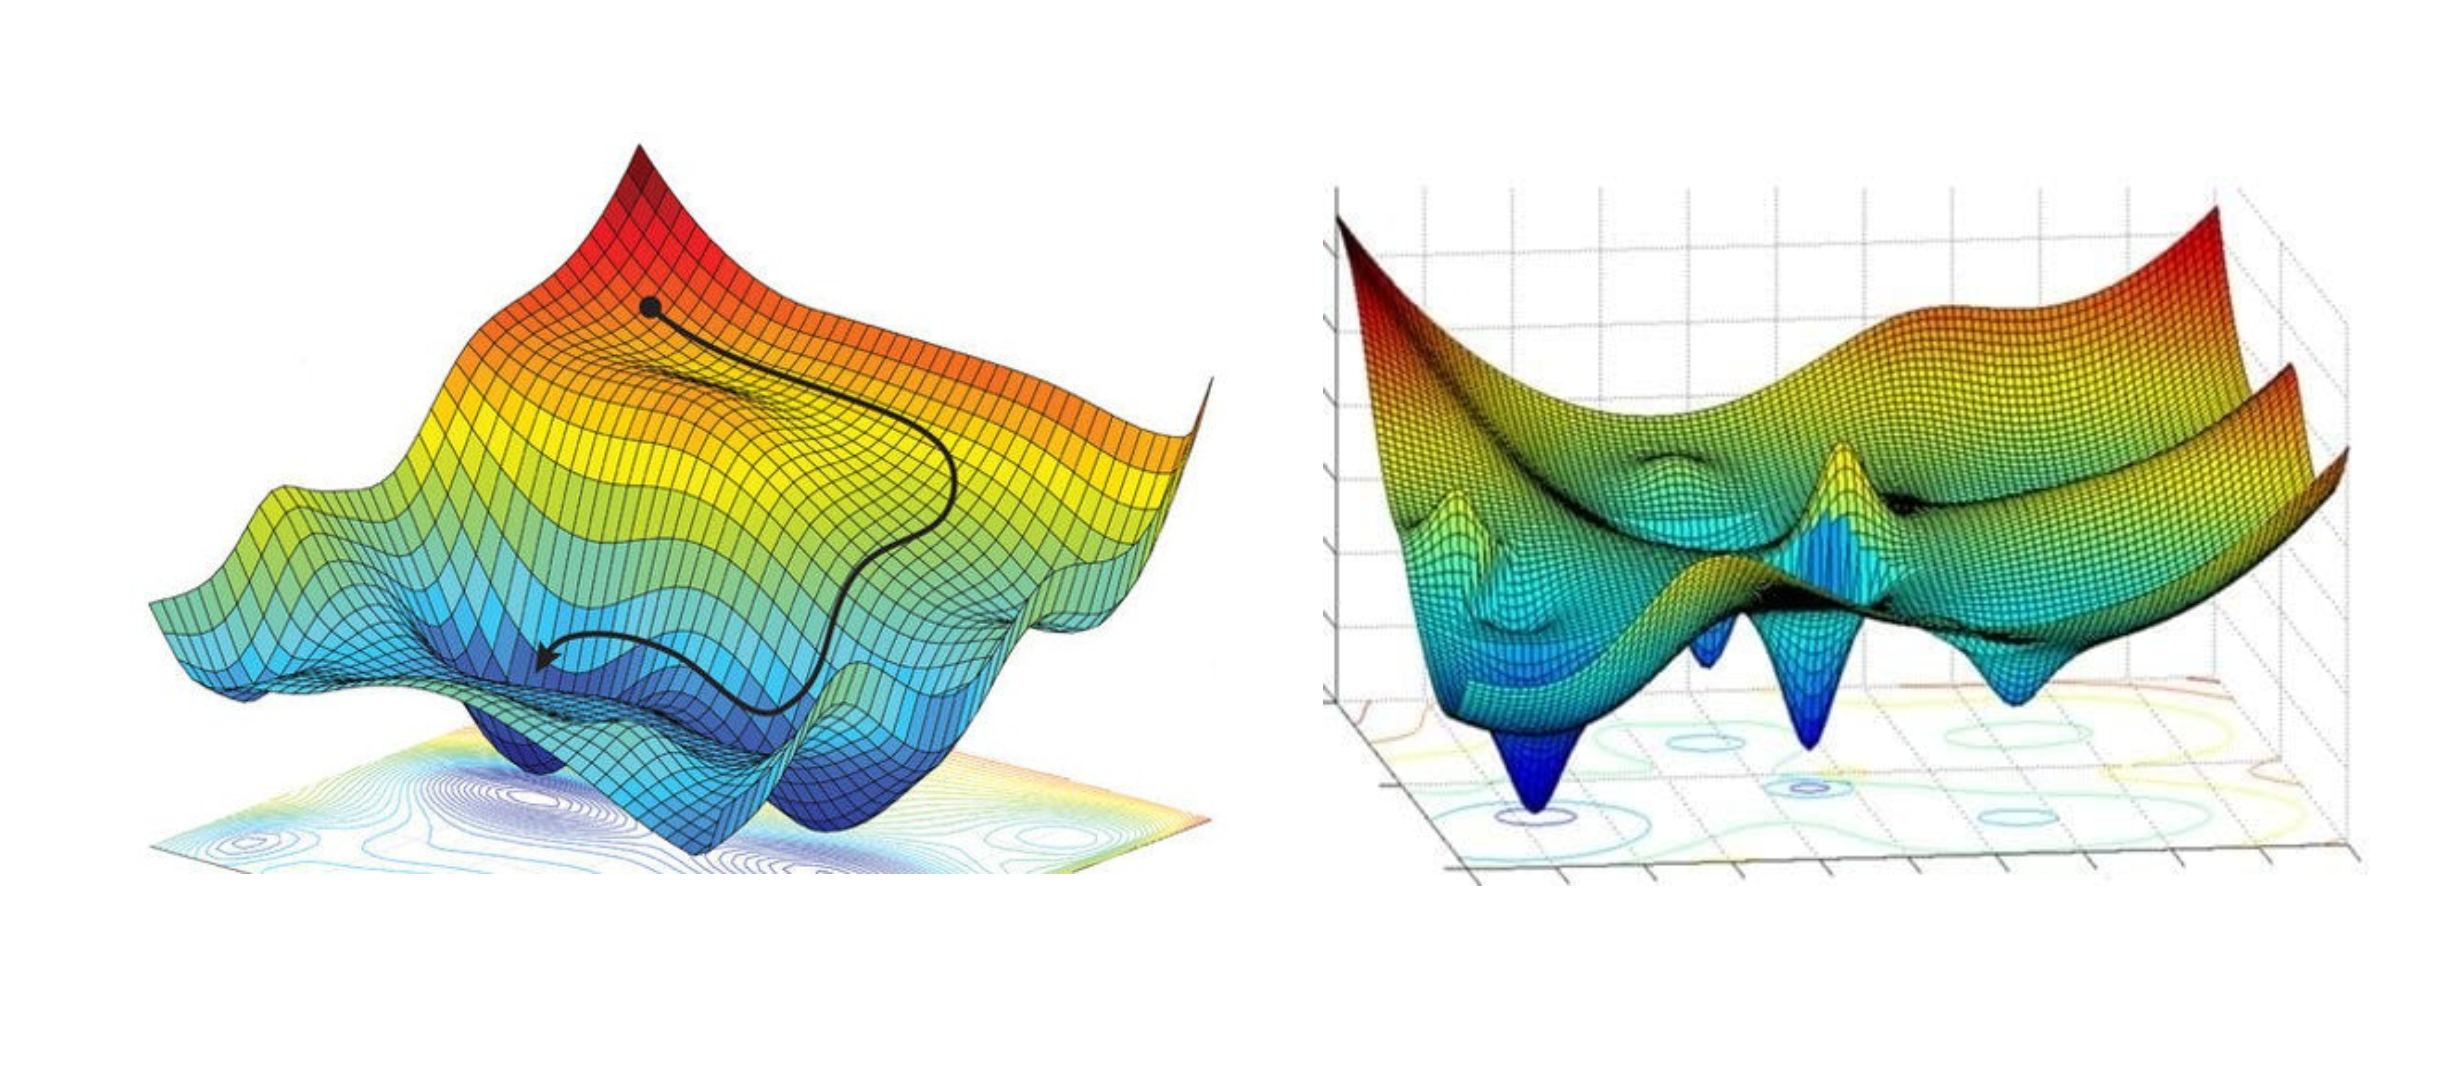
\includegraphics[width=\textwidth]{sgd.png}
\end{center}

\centerline{Dado $G$, ¿cuáles son los mínimos locales de $\mathcal E_G$?}

}

% \frame{\frametitle{Geometría del paisaje en alta dimensión}
%
% \begin{center}
% \includegraphics[width=\textwidth]{sgdcross.png}
% \end{center}
%
% Dado $G$, ¿cuáles son los mínimos locales de $\mathcal E_G$? ¿Bases de atracción?
% }

\setbeamercolor{background canvas}{bg=crema}

\frame{\frametitle{Modelo de Kuramoto}



{\bf\underline{Sincronización Global}}

\begin{center}
El único mínimo local de $\mathcal E_G$ es $\theta_u = \theta_v$ para todo $u,v \in V$.

\end{center}
}


\frame{\frametitle{Sincronización global: ¿cuánta conectividad hace falta?}
\beamerdefaultoverlayspecification{}

%{\bf \underline{Def.:}} $G$ \emph{sincroniza globalmente} si los únicos mínimos locales de $\mathcal E_G$ son los estados sincronizados.

\pause
\bigskip
\punto El grafo completo $K_n$ sincroniza globalmente (ejercicio).\\[4pt]
\punto Intuición: más aristas $\Rightarrow$ más fácil sincronizar \pause (\textbf{\underline{falso!}}).

\pause
\bigskip
\textbf{Conectividad:}\quad $\mu(G) = \dfrac{\min_{v\in V}\deg(v) + 1}{n}$.

\pause
\bigskip
\textbf{Conectividad crítica:}\quad $\mu_c = \inf\bigl\{\mu \;:\; \text{\emph{todo} grafo con } \mu(G)\ge\mu \text{ sincroniza globalmente}\bigr\}$.

}


\frame{\frametitle{¿Cuánto vale $\mu_c$?}
\beamerdefaultoverlayspecification{}

\centering
\begin{tikzpicture}[x=40cm, y=1cm, font=\footnotesize]
  % eje
  \draw[pizarra, line width=1pt, -{Stealth[length=6pt]}] (0,0) -- (0.365,0);
  \foreach \v/\t in {0.7/0{.}7, 0.8/0{.}8, 0.9/0{.}9, 1.0/1} {
    \draw[pizarra] ({\v-0.65},0.08) -- ({\v-0.65},-0.08);
    \node[pizarra, below] at ({\v-0.65},-0.08) {$\t$};
  }
  \node[pizarra, right] at (0.365,0) {$\mu$};
  \node[ambar!85!black, anchor=west, font=\small\bfseries] at (0,2.7) {Cotas superiores};

  % cotas superiores (arriba)
  \uncover<1->{
    \fill[ambar] ({1.0-0.65},0) circle (2.6pt);
    \node[above, align=center] at ({1.0-0.65},0.15) {$K_n$\\ (ejercicio)};
  }
  \uncover<2->{
    \fill[ambar] ({0.9395-0.65},0) circle (2.6pt);
    \node[above, align=center] at ({0.9395-0.65},0.15) {$0{.}9395$\\ Taylor 2012};
  }
  \uncover<3->{
    \fill[ambar] ({0.7929-0.65},0) circle (2.6pt);
    \fill[ambar] ({0.7889-0.65},0) circle (2.6pt);
    \node[above, align=center] at ({0.791-0.65},0.15) {$\approx 0{.}79$\\ Ling--Xu--Bandeira 2019\\ Lu--Steinerberger 2020};
  }
  \uncover<4->{
    \fill[ambar] ({0.75-0.65},0) circle (2.6pt);
    \draw[ambar, thin] ({0.75-0.65},0.1) -- ({0.75-0.65},1.55);
    \node[above, align=center] at ({0.75-0.65},1.5) {$3/4$\\ Kassabov--Strogatz--Townsend 2021};
  }
  % cotas inferiores (abajo)
  \uncover<5->{
    \fill[colresorte] ({0.6828-0.65},0) circle (2.6pt);
    \fill[colresorte] ({0.6838-0.65},0) circle (2.6pt);
    \fill[noche] ({0.6875-0.65},0) circle (2.6pt);
    \draw[colresorte, thin] ({0.6875-0.65},-0.1) -- ({0.6875-0.65},-0.65);
    \node[anchor=north west, align=left] at (0.0,-0.65)
      {{\small\bfseries\color{colresorte} Cotas inferiores:} $0{.}6828 \to 0{.}6838 \to 11/16 = 0{.}6875$\\ Townsend--Stillman--Strogatz 2020, Yoneda--Tatsukawa--Teramae 2021, Canale 2022};
  }
  % el intervalo y la conjetura
  \only<6>{
    \fill[ambar, opacity=0.3] ({0.6875-0.65},-0.07) rectangle ({0.75-0.65},0.07);
    \node[font=\small, align=left, anchor=north west] at (0,-1.75)
      {\textbf{Conjetura} (Bandeira et al., 2025): $\mu_c = 3/4$.};
  }
  \only<7->{
    \fill[ambar, opacity=0.3] ({0.6875-0.65},-0.07) rectangle ({0.742-0.65},0.07);
    \draw[ambar!85!black, line width=1.4pt] ({0.742-0.65},0.2) -- ({0.742-0.65},-0.2);
    \node[font=\Large\bfseries, ambar!85!black] at ({0.715-0.65},0.45) {?};
    \node[font=\small, align=left, anchor=north west] at (0,-1.75)
      {\textbf{Agosto 2026} (Lepsveridze--Zhang): $\mu_c \le 3/4 - \eta$.\quad \alert{\textbf{¡La conjetura es falsa!}}};
  }
\end{tikzpicture}

}


% Cierre
\begin{frame}[plain]
\begin{tikzpicture}[remember picture, overlay]
  \fill[noche] (current page.south west) rectangle (current page.north east);
  \coordinate (C) at ([xshift=-3.4cm]current page.east);
  \draw[colresorte, line width=1pt] (C) circle (2.3cm);
  \luciernagas{C}{2.3}{12}{7}
  \node[anchor=west, text width=9cm, text=crema, align=left]
    at ([xshift=1.1cm]current page.west) {%
    {\fontsize{28}{34}\selectfont $\dfrac{11}{16}\;\le\;\mu_c\;\le\;\dfrac34-\eta$}\par
    \vspace{6pt}{\color{ambar}\rule{3cm}{1.5pt}}\par
    \vspace{8pt}{\large Un problema abierto.}\par
    \vspace{14pt}{\large\bfseries\color{ambar} Dos semanas para achicar el intervalo\\ \dots\ o para explicarlo mejor que nadie.}\par
    \vspace{14pt}{\small\color{crema!70} \textbf{A continuación}: más sincronización, las reglas del \\juego, y qué tiene que ver todo esto con Netflix\\ y los algoritmos de recomendación.}};
\end{tikzpicture}
\end{frame}


% S. Strogatz:  You’ve certainly chosen a challenging one! Who knows, perhaps some clever new idea, with or without AI, will finally crack it. Please give the students my warmest wishes. I’ll be rooting for them, and I hope the Researchthon is a tremendous success!

\end{document}
